\documentclass[12pt]{article}
\usepackage{a4wide}
\usepackage{latexsym}
\usepackage{amssymb}
\usepackage{epic}
\usepackage{amsmath}
\usepackage{graphicx}
\usepackage{comment}
\usepackage{graphicx}
\usepackage{tikz}
\usepackage{listings}
\usepackage{float}
\usepackage{xspace}

\newcommand{\tr}{\mbox{\sf true}}
\newcommand{\fa}{\mbox{\sf false}}
\newcommand{\beq}{\leftrightarrow}
\newcommand{\bimp}{\rightarrow}
\newcommand{\band}{\wedge}
\newcommand{\bor}{\vee}
\newcommand{\provernine}{\texttt{Prover9}\xspace}

\newcommand{\blue}[2]{\mathtt{blue}(#1, #2)}
\newcommand{\red}[2]{\mathtt{red}(#1, #2)}
\newcommand{\bluep}[2]{\mathtt{blue\_path}(#1, #2)}
\newcommand{\redp}[2]{\mathtt{red\_path}(#1, #2)}

\newcommand{\edge}[3]{\mathtt{edge}(#1, #2, #3)}
\newcommand{\path}[3]{\mathtt{path}(#1, #2, #3)}

\begin{document}
\section*{Automated Reasoning\\Assignment 3}

\begin{center}
Wouter Geraedts (s0814857)
\end{center}

\vspace{8mm}

\subsection*{Two-color reachability}

\paragraph{The problem}
Given an undirected graph where the edges are colored red and blue, use
\provernine to prove there exists a path from $A$ to $B$ such that no two
consecutive edges are of the same color.
Moreover, if given that certain edges exists, establish from the \provernine
output which path has been found.
\begin{figure}[H]
	\begin{center}
		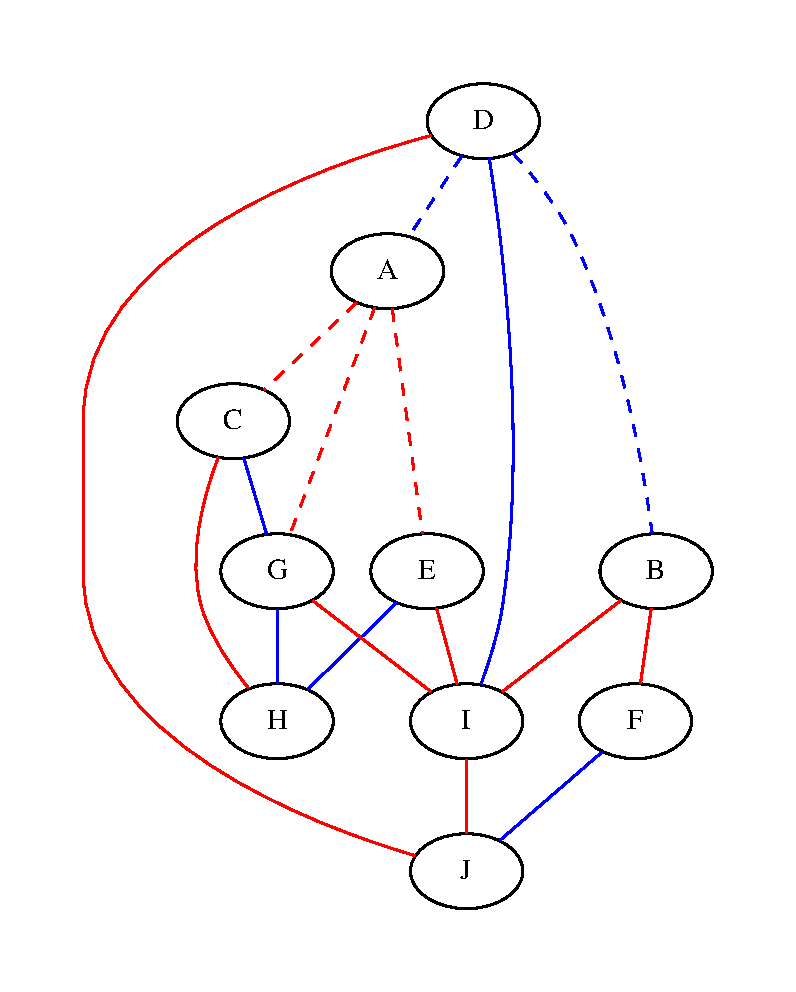
\includegraphics[width=0.6\textwidth]{graph.pdf}
	\end{center}
	\caption{The undirected bi-color graph as given in the assignment.}
\end{figure}

\paragraph{Solution}
Given nodes $A \ldots J$, I define these nodes as constants.
A blue edge between two nodes $x$ and $y$ is denoted by $\blue{x}{y}$,
and similarly for red edges by $\red{x}{y}$.
Thus the blue edge between $B$ and $F$ is denoted by $\blue{B}{F}$.
The uncertain edges are encoded with a disjunction:
\[ \red{A}{C} \bor \red{A}{E} \bor \red{A}{G} \]
\[ \blue{D}{A} \bor \blue{D}{B} \].
Because the graph is undirected, this edge relation is symmetric:
\[ \blue{x}{y} \bimp \blue{y}{x} \]
\[ \red{x}{y} \bimp \red{y}{x} \]
Now we introduce the notion of an alternating path from $x$ to $y$ ending with a blue edge:
$\bluep{x}{y}$, and similarly $\redp{x}{y}$.
A path ending in a blue edge, followed by a red edge, forms a path ending in a red edge:
\[ \bluep{x}{y} \band \red{y}{z} \bimp \redp{x}{z} \]
\[ \redp{x}{y} \band \blue{y}{z} \bimp \bluep{x}{z} \]
Finally, the empty path is valid in itself, thus the path relation is reflexive:
\[ \bluep{x}{x} \band \redp{x}{x} \]

Now we only need to prove the existance of the path from $A$ to $B$, by adding
a \provernine goal:
\[ \bluep{A}{B} \bor \redp{A}{B} \]
Which \provernine reports to be true, and yields a proof for within 0.008 seconds.
The proof is composed of 39 steps.

\paragraph{Solution for fixed edges}
The uncertain edges are now replaced with $\red{A}{E}$ and $\blue{B}{D}$.
Running this model in \provernine however does not terminate within a reasonable amount of time.
Analysis shows that the symmetry rules for the edges cause this behaviour.
Removing the edge symmetry property, and folding this aspect into the path relation,
allows \provernine to solve the model:
\[ \bluep{x}{y} \band (\red{y}{z} \bor \red{z}{y}) \bimp \redp{x}{z} \]
\[ \redp{x}{y} \band (\blue{y}{z} \bor \blue{z}{y}) \bimp \bluep{x}{z} \]
This yields a proof within 0.006 seconds.
The proof is composed of 37 steps.

Extracting the used edges from the proof is simple:
only the edges used in the construction of the path show up in the proof itself,
as listed in figure \ref{fig:proof-assump}, and drawn in figure \ref{fig:proof-graph}.
\begin{figure}[H]
	\begin{center}
		\begin{lstlisting}[frame=single]
10 red(B,F).  [assumption].
12 red(C,H).  [assumption].
13 red(D,J).  [assumption].
14 red(E,I).  [assumption].
15 red(G,I).  [assumption].
17 blue(C,G).  [assumption].
18 blue(D,I).  [assumption].
19 blue(E,H).  [assumption].
20 blue(F,J).  [assumption].
		\end{lstlisting}
	\end{center}
	\caption{\label{fig:proof-assump} All edges in the proof of the aforementioned model.}
\end{figure}
\begin{figure}[H]
	\begin{center}
		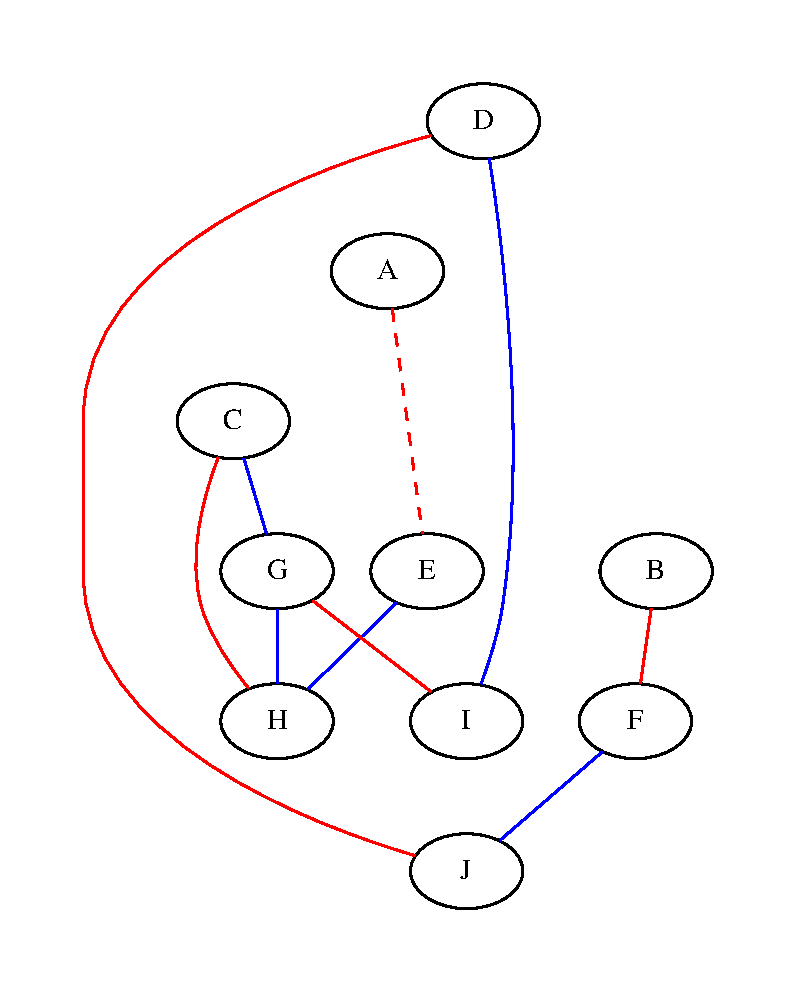
\includegraphics[width=0.4\textwidth]{graph-fixed.pdf}
	\end{center}
	\caption{\label{fig:proof-graph} The graph constructed from the aforementioned edges.}
\end{figure}

\paragraph{Generalization}
I generalized the solution to solve the $n$-color reachability problem
by parameterizing the edge and path relations in the color of the path and edge:
\[ \forall c_1, c_2 ~.~ c_1 \neq c_2 \bimp (\path{x}{y}{c_1} \band ( \edge{y}{z}{c_2} \bor \edge{z}{y}{c_2} ) \bimp \path{x}{z}{c_2} ) \]
Similarly I adapt reflexivity for the $\mathtt{path}$ relation.
\[ \forall c ~.~ \path{x}{x}{c} \]
The uniqueness of colors now still needs to be defined.
There is no easy way to define a set of objects in \provernine, and state
that each element is unique.
So for every pair, we then need to define inequality, like this:
\[ \mathtt{Blue} \neq \mathtt{Red} \]
And finally the goal can be defined as follows:
\[ \exists c ~.~ \path{A}{B}{c} \]

I applied this generalization to a random 3-color graph, as seen in figure \ref{fig:graph2}. \\

\noindent
\begin{minipage}[b]{\textwidth}
	\begin{minipage}[b]{0.50\textwidth}
		\begin{figure}[H]
			\begin{center}
				\includegraphics[width=0.8\textwidth]{graph2.pdf}
			\end{center}
			\caption{\label{fig:graph2} A random 3-color graph.}
		\end{figure}
	\end{minipage}
	\begin{minipage}[b]{0.50\textwidth}
		\begin{figure}[H]
			\begin{center}
				\includegraphics[width=0.8\textwidth]{graph2-solved.pdf}
			\end{center}
			\caption{\label{fig:graph2} The 3-color graph as solved by \provernine.}
		\end{figure}
	\end{minipage}
\end{minipage}

\end{document}
